\documentclass{beamer}

\title{Formation KI} % Titre du rapport ou matière
\subtitle{Python} % Sous-titre du rapport
\author{Yann Lapous (KI 025)}
\date{4 sept 2023}

\usepackage[utf8]{inputenc}
\usepackage[T1]{fontenc}
\usepackage[french]{babel}
\usepackage{svg}
\usepackage{tcolorbox}
\usepackage{xcolor}
\usepackage{listings}
\usepackage{appendix}
\usepackage{appendixnumberbeamer}
\usepackage{pgfplots}
\usepackage{qrcode}
\usepackage{fontawesome5}


\pgfplotsset{compat=1.18}

\usetheme{CambridgeUS}

% Définition de quelques couleurs (bleu du logo des Ponts)
\definecolor{bleuPonts}{HTML}{0194C6}

% Définition des couleurs du thème
\setbeamercolor{section in toc}{fg=black,bg=white}
\setbeamercolor{alerted text}{fg=red!80!gray}
\setbeamercolor*{palette primary}{fg=bleuPonts!60!black,bg=gray!30!white}
\setbeamercolor*{palette secondary}{fg=bleuPonts!70!black,bg=gray!15!white}
\setbeamercolor*{palette tertiary}{bg=bleuPonts!80!black,fg=gray!10!white}
\setbeamercolor*{palette quaternary}{fg=bleuPonts,bg=gray!5!white}

\setbeamercolor*{sidebar}{fg=red,bg=gray!15!white}
%set color structure
\setbeamercolor*{structure}{fg=bleuPonts!80!black}

\setbeamercolor*{palette sidebar primary}{fg=bleuPonts!10!black}
\setbeamercolor*{palette sidebar secondary}{fg=gray!10!blak}
\setbeamercolor*{palette sidebar tertiary}{fg=bleuPonts!50!black}
\setbeamercolor*{palette sidebar quaternary}{fg=gray!30!blak}

%\setbeamercolor*{titlelike}{parent=palette primary}
\setbeamercolor{titlelike}{parent=palette primary,fg=bleuPonts}
\setbeamercolor{frametitle}{bg=gray!10!white}
\setbeamercolor{frametitle right}{bg=gray!60!white}

\setbeamercolor*{separation line}{}
\setbeamercolor*{fine separation line}{}

% Définition de la page de garde
\defbeamertemplate*{title page}{customized}[1][]
{
    \centering
    \includesvg[width=0.2\paperwidth]{assets/logo.svg}\par
    \bigskip
    \usebeamerfont{title}\Huge{\inserttitle}\par
    \usebeamerfont{subtitle}\usebeamercolor[fg]{subtitle}\Large{\insertsubtitle}\par
}

% Définition de la forme des items
\setbeamertemplate{itemize items}[default]
\setbeamertemplate{enumerate items}[default]
\setbeamertemplate{section in toc}[square]

% Enlève la barre de navigation
\beamertemplatenavigationsymbolsempty

% Couleurs pour les listings (Dracula)
\definecolor{draculaBackground}{HTML}{282a36}
\definecolor{draculaCurentLine}{HTML}{44475a}
\definecolor{draculaSelection}{HTML}{44475a}
\definecolor{draculaForeground}{HTML}{f8f8f2}
\definecolor{draculaComment}{HTML}{6272a4}
\definecolor{draculaCyan}{HTML}{8be9fd}
\definecolor{draculaGreen}{HTML}{50fa7b}
\definecolor{draculaOrange}{HTML}{ffb86c}
\definecolor{draculaPink}{HTML}{ff79c6}
\definecolor{draculaPurple}{HTML}{bd93f9}
\definecolor{draculaRed}{HTML}{ff5555}
\definecolor{draculaYellow}{HTML}{f1fa8c}
%utilisation pour les listings de ces couleurs
% \lstset{
%     frame=tb,
%     basicstyle=\ttfamily\tiny\color{draculaForeground},
%     backgroundcolor=\color{draculaBackground},
%     commentstyle=\color{draculaComment},
%     keywordstyle=\color{draculaCyan},
%     stringstyle=\color{draculaGreen},
%     identifierstyle=\color{draculaPink},
%     breaklines=true,
%     numbers=left,
%     numberstyle=\color{bleuPonts},
%     extendedchars=true,
%     xleftmargin=5mm,
%     xrightmargin=5mm
% }

\definecolor{codegreen}{rgb}{0,0.6,0}
\definecolor{codegray}{rgb}{0.5,0.5,0.5}
\definecolor{codepurple}{rgb}{0.58,0,0.82}
\definecolor{backcolour}{rgb}{0.95,0.95,0.92}

\lstdefinestyle{mystyle}{
    backgroundcolor=\color{backcolour},   
    commentstyle=\color{codegreen},
    keywordstyle=\color{magenta},
    numberstyle=\tiny\color{codegray},
    stringstyle=\color{codepurple},
    identifierstyle=\color{blue},
    basicstyle=\ttfamily\scriptsize,
    breakatwhitespace=false,         
    breaklines=true,                 
    captionpos=b,                    
    keepspaces=true,                 
    numbers=left,                    
    numbersep=5pt,                  
    showspaces=false,                
    showstringspaces=false,
    showtabs=false,                  
    tabsize=2
}

\lstset{style=mystyle}

\begin{document}
    \begin{frame}
        \titlepage
    \end{frame}

    \begin{frame}
        \frametitle{Sommaire}
        \setcounter{tocdepth}{1}
        \tableofcontents
    \end{frame}
    \section*{Introduction}
    \begin{frame}
        \frametitle{Pourquoi cette formation ?}
        \centering
        
\includegraphics[width=.5\textwidth]{assets/meme_python.png}
    \end{frame}
    \begin{frame}
        \centering

        \normalsize\url{https://kiclubinfo.notion.site/Formation-Python-219ab0fc71c24f50b06bee30f60f649a?pvs=4}
	\\[.5cm]
        \qrcode[height=.3\textwidth]{https://kiclubinfo.notion.site/Formation-Python-219ab0fc71c24f50b06bee30f60f649a?pvs=4}
    \end{frame}
    
    \section{Base du langage}
    \subsection{Variables}
    \begin{frame}
        \frametitle{Types de variables}
        \lstinputlisting[language=python]{assets/pres_var.py}

        \begin{itemize}
            \item \texttt{int} pour les \textbf{entier}
            \item \texttt{float} pour les \textbf{décimaux}
            \item \texttt{bool} pour les \textbf{booléen}
            \item \texttt{string} pour les \textbf{chaines de caractères}
        \end{itemize}
    \end{frame}
    \begin{frame}
        \frametitle{Opérations et relations binaires}
        \begin{itemize}
            \item \texttt{x+y} : \textbf{Addition}
            \item \texttt{x-y} : \textbf{Soustraction}
            \item \texttt{x*y} : \textbf{Multiplication}
            \item \texttt{x/y} : \textbf{Division}, renvoie (toujours) un flottant
            \item \texttt{x//y} : \textbf{Quotient}
            \item \texttt{x\%y} : \textbf{Reste}
            \item \texttt{x==y} : \textbf{\'Egalité}
            \item \texttt{<},\texttt{<=},\texttt{>} et \texttt{>=} : \textbf{Relation d'ordre}
        \end{itemize}
    \end{frame}
    \subsection{Listes et dictionnaires}
    \begin{frame}
        \frametitle{Listes}
        \lstinputlisting[language=python]{assets/liste.py}
    \end{frame}
    \begin{frame}
        \frametitle{Dictionnaires}
        \lstinputlisting[language=python]{assets/dico.py}
    \end{frame}
    \subsection{Boucles et conditions}
    \begin{frame}
        \frametitle{Conditions}
        \lstinputlisting[language=python]{assets/condition.py}
    \end{frame}
    \begin{frame}
        \frametitle{Boucle \texttt{while}}
        \lstinputlisting[language=python]{assets/while.py}
    \end{frame}
    \begin{frame}
        \frametitle{Boucle \texttt{for}}
        \lstinputlisting[language=python]{assets/for.py}
    \end{frame}
    \subsection{Fonctions}
    \begin{frame}
        \frametitle{Fonctions réutilisables}
        \lstinputlisting[language=Python]{assets/fonct.py}
    \end{frame}
    \begin{frame}
        \lstinputlisting[language=Python]{assets/fonc2.py}
    \end{frame}

    \section{Programmation orientée objet}
    \begin{frame}
        \frametitle{La POO c'est quoi ?}
        \centering
        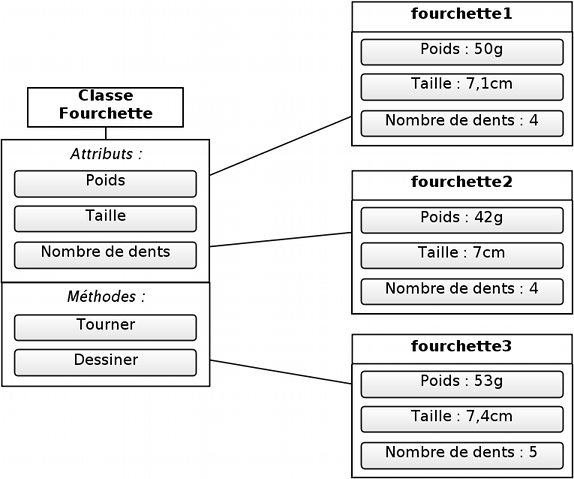
\includegraphics[width=.7\textwidth]{assets/schéma_poo.png}
    \end{frame}
    \subsection{Définir une classe}
    \begin{frame}
        \frametitle{Initialisation}
        \lstinputlisting[language=Python]{assets/poo_init.py}
    \end{frame}
    \begin{frame}
        \frametitle{Méthodes}
        \lstinputlisting[language=Python]{assets/poo_methodes.py}
    \end{frame}

    \section{Modules importants}
    \begin{frame}
        \frametitle{Quelques modules}
        \begin{itemize}
            \item \faCalculator \ \textbf{\textit{NumPy}} : Bibliothèque  qui permet de manipuler des matrices ou tableaux multidimensionnels ainsi que des fonctions mathématiques opérant sur ces tableaux.
            \item \faChartBar \ \textbf{\textit{Matplotlib}} : Bibliothèque destinée à tracer et visualiser des données sous forme de graphiques.
            \item \faTable \ \textbf{\textit{Pandas}} : Bibliothèque permettant la manipulation et l'analyse des données.
        \end{itemize}

        \begin{block}{Utilisation (exemple avec \textit{NumPy})}
            On place au début de son script la ligne suivante :
            \lstinline[language=Python]{import numpy as np} 

            On utilise les différentes fonction en appliquant \lstinline[language=Python]{np.} puis la fonction (ou constructeur d'objet). Exemple : \lstinline[language=Python]{np.array([2,3,4])} ou \lstinline[language=Python]{np.sqrt(9)}

        \end{block}
    \end{frame}

    \section*{Conclusion}
    \begin{frame}
        \centering
        \Huge Merci, à vous de jouer !
        
        \vspace{1cm}

        \normalsize\url{https://kiclubinfo.notion.site/Formation-Python-219ab0fc71c24f50b06bee30f60f649a?pvs=4}

        \vspace{.5cm}
        \qrcode[height=.3\textwidth]{https://kiclubinfo.notion.site/Formation-Python-219ab0fc71c24f50b06bee30f60f649a?pvs=4}
    \end{frame}

\end{document}
